\section{Erweiterte Partitionierung: Partitionen formatieren}
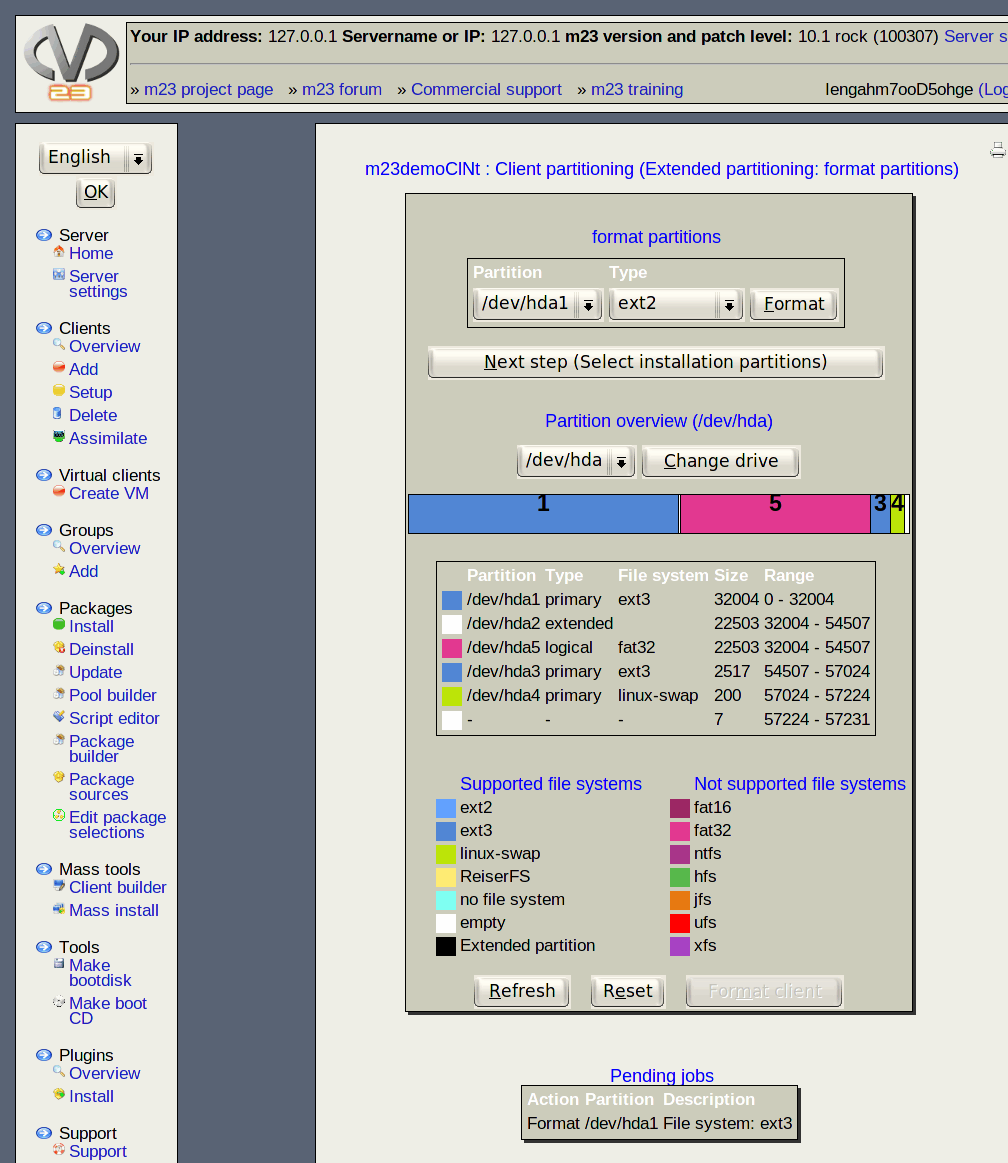
\includegraphics[scale=0.4]{/mdk/doc/manual/screenshots/de/fdisk-extended2.png} \\
\begin{itemize}
\item W�hlen Sie die Partition, die Sie formatieren m�chten, indem Sie den Typ des Dateisystems bestimmen und auf \textit{"Formatieren"} klicken. Zur Wahl des "richtigen" Dateisystems lesen Sie die Information am Ende der Seite.\\
\item Haben Sie alle gew�nschten Partitionen formatiert, so klicken Sie auf \textit{""}.\\
\end{itemize}
\subsection{Hinweis}
Sie ben�tigen mindestens eine ext2-, ext3- oder reiserfs-formatierte Partition und zus�tzlich eine Partition mit linux-swap-Dateisystem, um die Installation zu beginnen.\\
\subsection{Information: Dateisysteme}
\begin{itemize}
\item \textbf{ext2:} ein �lteres Dateisystem, geeignet zum Installieren des Basissystems\\
\item \textbf{ext3(empfohlen), reiserfs}: neuere Journaling-Dateisysteme, die zum Installieren des Basissystems geeignet sind\\
\item \textbf{linux-swap:} wird zum Anlegen des Linux-Swap-Speichers verwendet.\\
\end{itemize}
